\chapter{Metodología de la Investigación}

( Hablar sobre la metodología, como crear nubes, verificar calidad, explicar los test )

\section{Nube de aproximación}

Triangulación de Delaunay

\subsection{Criterio de creación de nube}

\subsection{Verificación de la calidad de la nube}
Para verificar la calidad de la nube se implementan dos pruebas, la primera consiste en verificar el cumplimiento de las condiciones de consistencia, es decir, (*****)

\begin{eqnarray} \label{eq:d0_consistency_conditions}
    \sum_{i=1}^{np} \phi_i - 1 = 0 \\
    \sum_{i=1}^{np} \phi_i \vec{x}_i = \vec{x}
\end{eqnarray}

\begin{eqnarray} \label{eq:d1_consistency_conditions}
    \sum_{i=1}^{np} \frac{\partial{\phi_i}}{\partial{\vec{x}}} = \vec{0} \\
    \sum_{i=1}^{np} \frac{\partial\{\phi_i\vec{x}_i\}}{\partial\vec{x}} - \textbf{Id} = \textbf{0} 
\end{eqnarray}

\begin{eqnarray} \label{eq:d2_consistency_conditions}
    \sum_{i=1}^{np} \frac{\partial^2{\phi_i}}{\partial x^2} = \textbf{0} \\
    \sum_{i=1}^{np} \frac{\partial^2\{\phi_i\vec{x}_i\}}{\partial\vec{x}^2} = \mathbb{M}_0 
\end{eqnarray}
donde $\mathbb{M}_0$ es un tensor nulo de orden 3

Mediante una aproximación de espacios convexo se verifica la calidad de la aproximación, la función de forma debiera aproximar :
\begin{eqnarray}
    \sum_{i=1}^{np} f(\vec{x}_i) \phi_i(\vec{x}) - f(\vec{x}) = 0 \\
    \sum_{i=1}^{np} \frac{\partial\{f(\vec{x}_i)\phi_i(\vec{x})\}}{\partial \vec{x}} - \frac{\partial f(\vec{x})}{\partial \vec{x}} = \vec{0} \\
    \sum_{i=1}^{np} \frac{\partial^2\{f(\vec{x}_i)\phi_i(\vec{x})\}}{\partial \vec{x}^2} - \frac{\partial^2 f(\vec{x})}{\partial \vec{x}^2} = \textbf{0}
\end{eqnarray}
Se utiliza la siguiente función como test:
\begin{equation}
    f(\vec{x}) = \vec{x} \cdot \vec{x}
\end{equation}
es decir, $x^2$ y $x^2+y^2$ en 1D y 2D respectivamente.


\subsection{Generación de nube}
Entre las alternativas para generar nubes de aproximación se encuentran (citar a rainald). En este trabajo se utilizó el algoritmo propuesto por Rainald (citar libro), rutina que crea una colección de puntos discretos cercanos previamente triangulados (Triangulación de Delaunay).


\begin{figure}
    \centering
    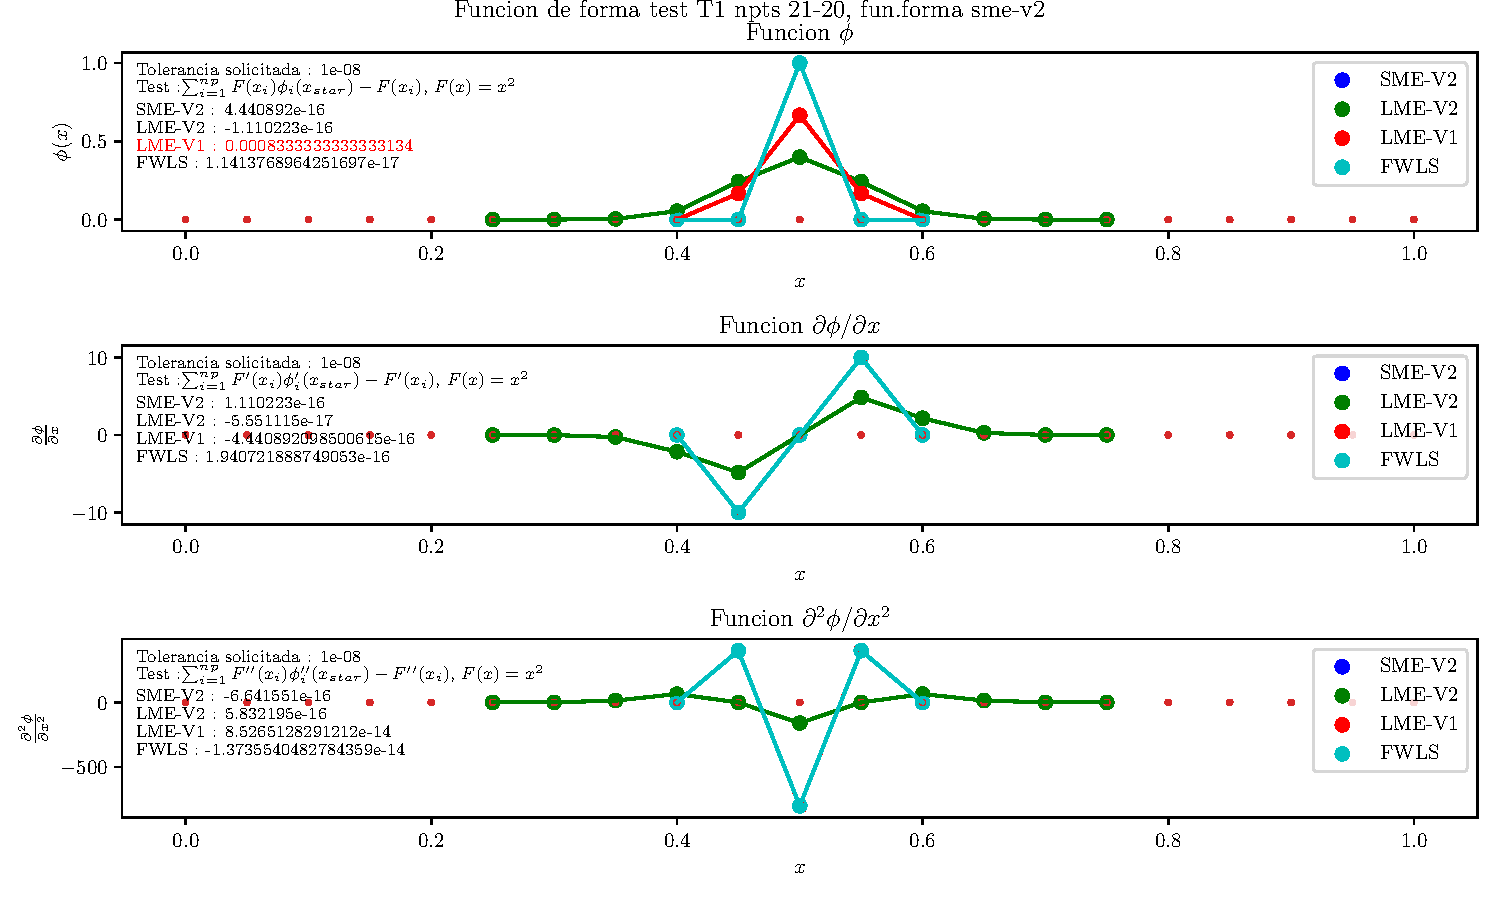
\includegraphics[width=1\textwidth]{./Imagenes/05/T1_21-20_regular_type-2_direct_10.pdf}
    \caption{Gráfica de las funciones de forma para una distribución regular} \label{fig:multiple_sf}
\end{figure}

\begin{figure}
    \centering
    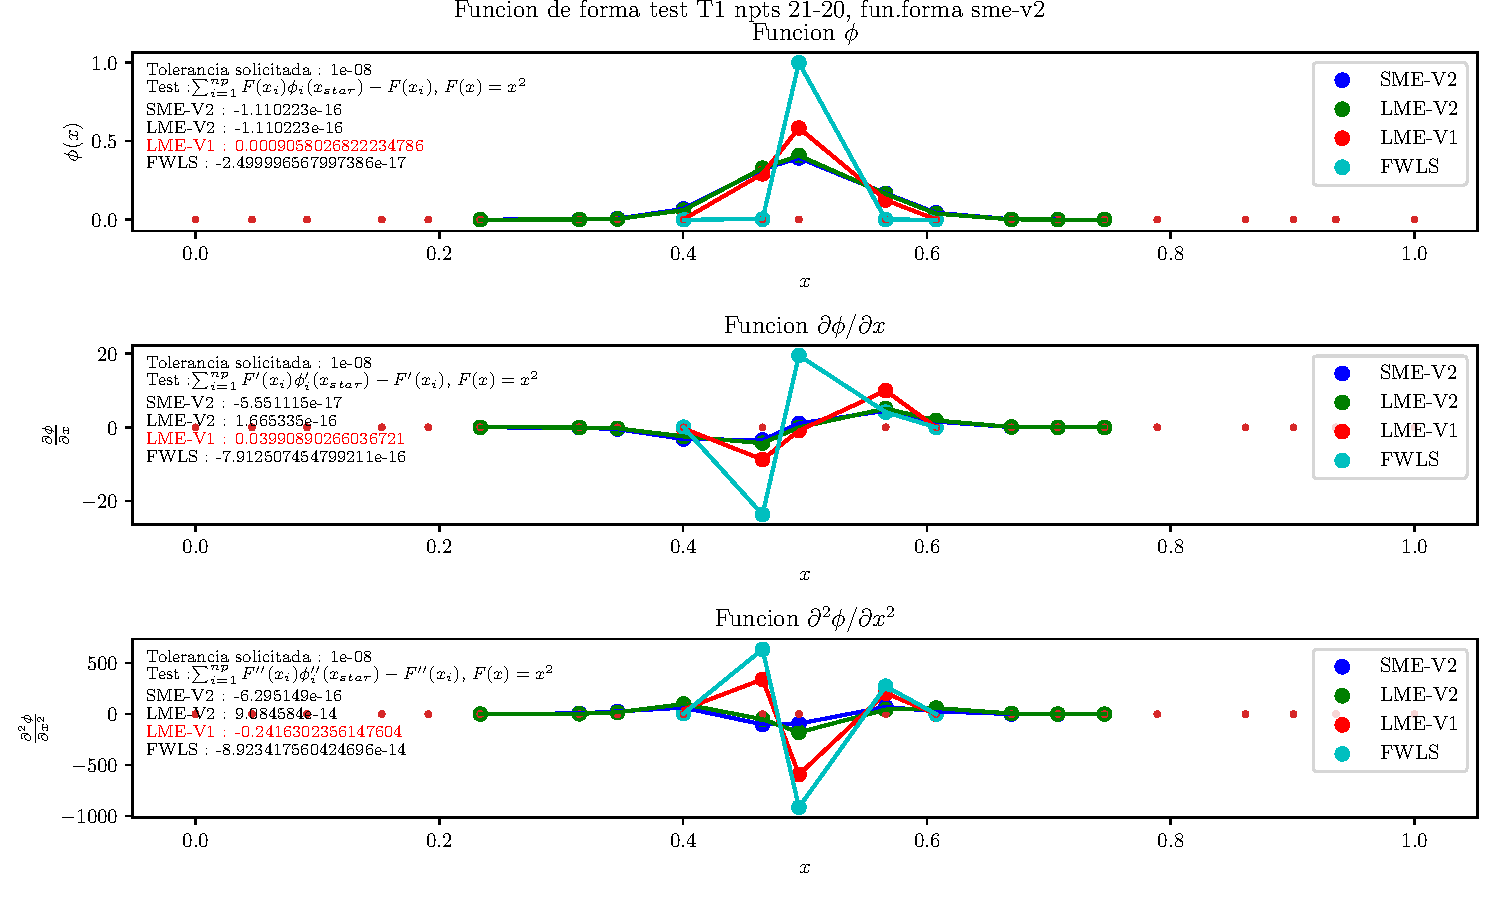
\includegraphics[width=1\textwidth]{./Imagenes/05/T1_21-20_irreg_type-2_direct_10.pdf}
    \caption{Gráfica de las funciones de forma para una distribución irregular} \label{fig:multiple_sf}
\end{figure}


